\documentclass[12pt, twoside]{article}
% \documentclass[12pt, twoside]{article}
\usepackage[letterpaper, margin=1in, headsep=0.2in]{geometry}
\setlength{\headheight}{0.6in}
%\usepackage[english]{babel}
\usepackage[utf8]{inputenc}
\usepackage{microtype}
\usepackage{amsmath}
\usepackage{amssymb}
%\usepackage{amsfonts}
\usepackage[nomessages]{fp} %\FPeval{\var-name}{2*sin(pi/6)}
\usepackage{siunitx} %units in math. eg 20\milli\meter
\usepackage{yhmath} % for arcs, overparenth command
\usepackage{tikz} %graphics
\usetikzlibrary{quotes, angles, arrows, arrows.meta}
\usepackage{graphicx} %consider setting \graphicspath{{images/}}
\usepackage{parskip} %no paragraph indent
\usepackage{enumitem}
\usepackage{multicol}
\usepackage{venndiagram}

\usepackage{fancyhdr}
\pagestyle{fancy}
\fancyhf{}
\renewcommand{\headrulewidth}{0pt} % disable the underline of the header
\raggedbottom
\hfuzz=2mm %suppresses overfull box warnings

\usepackage{hyperref}
\usepackage{float}

\fancyhead[LE]{\thepage}
\fancyhead[RO]{\thepage \\ First and last name: \hspace{2.5cm} \,\\ Section: \hspace{2.5cm} \,}
\fancyhead[LO]{BECA/Huson/Geometry: Solid geometry \\* 12 February 2025}

\begin{document}
\subsubsection*{5.5 Exam: Cumulative Review}
\begin{enumerate}[itemsep=0.5cm]
\item Point $G$ bisects $\overline{FH}$, with $FG=3x - 3$, $FH=36$. Find $x$. \par \medskip
  \begin{tikzpicture}
      \draw[fill] (0,0) circle [radius=0.05] node[below]{$F$};
      \draw[-, thick] (0,0)--(8,0);
      \draw[fill] (4,0) circle [radius=0.05] node[below]{$G$};
      \draw[fill] (8,0) circle [radius=0.05] node[below]{$H$};
      \node at (2,0.5) [above]{$3x - 3$};
      \node at (4,-0.75) [below]{$36$};
      \draw (1.8,-0.2)--(1.9,0.2);
      \draw (2.1,-0.2)--(2.2,0.2);
      \draw (5.8,-0.2)--(5.9,0.2);
      \draw (6.1,-0.2)--(6.2,0.2);
  \end{tikzpicture} \vspace{2cm}

\subsubsection*{G.CO.12 Make and justify formal geometric constructions}
\item Construct an equilateral triangle with side $\overline{PQ}$.  
  \vspace{1cm}
  \begin{flushleft}
  \begin{tikzpicture}
    \draw [-, thick] (0,0)--(0,-4);
    \draw [fill] (0,0) circle [radius=0.05] node[above]{$P$};
    \draw [fill] (0,-4) circle [radius=0.05] node[below]{$Q$};
  \end{tikzpicture}
  \end{flushleft} 
  \vspace{0.5cm}

\item Construct the angle bisector of $\angle A$.  
  \vspace{1cm}
  \begin{flushright}
  \begin{tikzpicture}
    \draw [<->, thick] (-6,1)--(0,0)--(4,4);
    \draw [fill] (0,0) circle [radius=0.05] node[below left]{$A$};
  \end{tikzpicture}
  \end{flushright} 
  %\vspace{3cm}
      
\newpage
\subsubsection*{G.CO.5 Transform a figure using translation, reflection, or rotation}
\item  Rotate $\triangle ABC$ $90^\circ$ clockwise around the origin. Label the image $\triangle A'B'C'$.
    \begin{center}
      \begin{tikzpicture}[scale=0.6]
        \draw [help lines] (-8,-7) grid (8,7);
        \draw [thick, <->] (-8.4,0) -- (8.4,0) node [below right] {$x$};
        \draw [thick, <->] (0,-7.4)--(0,7.4) node [left] {$y$};
        \draw [thick] (0,3) node[left] {$A$}--
          (2,1) node[above right] {$B$}--
          (2,5) node[above right] {$C$}--
          cycle;
      \end{tikzpicture}
      \end{center}
  
\item A translation maps $P(-7,-2) \rightarrow P'(-9,2)$. What is the image of $Q(-1,-3)$ under the same translation? \vspace{1cm}
      
\item The dilation mapping $x \rightarrow 2x$ and $y \rightarrow 2y$ is applied to $\triangle ABC$.
  \begin{enumerate}
    \item Write as coordinate pairs the vertices of the image, $\triangle A'B'C'$ \\[0.3cm]
    $A(-3,2) \rightarrow$ \\[0.7cm]
    $B(5,-2) \rightarrow$ \\[0.7cm]
    $C(6,0) \rightarrow$ \\[0.1cm]
    \item Which triangle is larger, or are they the same size? Justify your answer.
  \end{enumerate} \vspace{2cm}

\newpage
\item Apply a translation of up three and left five to $\triangle ABC$. Plot and label the image $\triangle A'B'C'$ on the axes below.
  \begin{center}
    \begin{tikzpicture}[scale=.7]
      \draw [help lines] (-8,-6) grid (8,8);
      \draw [thick, <->] (-8.4,0) -- (8.4,0) node [right] {$x$};
      \draw [thick, <->] (0,-6.4)--(0,8.4) node [above] {$y$};
      \draw [thick]
        (3,4) node[above right] {$A$}--
        (2,-1) node[below] {$B$}--
        (6,2) node[below] {$C$}--
        cycle;
    \end{tikzpicture}
  \end{center}

\item Dilate $\triangle ABC \rightarrow \triangle A'B'C'$ by a factor of $k=3$ centered at the origin, \\
$(x,y) \rightarrow (2x, 2y)$. Plot and label the image on the axes.
  \begin{center}
      \begin{tikzpicture}[scale=0.8]
      \draw [help lines] (-8,-3) grid (8,6);
      \draw [thick, <->] (-8.4,0) -- (8.4,0) node [right] {$x$};
      \draw [thick, <->] (0,-3.4)--(0,6.4) node [above] {$y$};  
      \draw [thick]
          (0,0) node[below right] {$A$}--
          (-2,2) node[above right] {$B$}--
          (-2, -1) node[below right] {$C$}--cycle;  
      \end{tikzpicture}
  \end{center}

\newpage
\subsubsection*{G.SRT.5 Use similarity criteria for triangles to solve problems}
\item Given $\triangle ABC \sim \triangle DEF$, $m\angle B=35^\circ$, and $m\angle C=100^\circ$. Find $m\angle D$. \vspace{4cm}


\item Similar triangles $\triangle ABP \sim \triangle JKP$ are shown with $P$ the intersection of $\overline{AJ}$ and $\overline{BK}$.
\begin{multicols}{2}
  \begin{enumerate}
      \item What line is parallel to $\overline{AB}$?
      \item If $AP = 10$, $BP = 6$, and $KP = 15$, what is the scale factor $k$? \vspace{2cm}
      \end{enumerate}
  \begin{tikzpicture}[rotate=-20, scale=1.4]
      \draw [thick]
        (-0.25,-1)node[below left]{$B$}--
        (0.5,2)node[left]{$K$}--
        (4,0)node[below left]{$J$}--
        (0,0)node[above]{$P$}--
        (-2,0)node[left]{$A$}--cycle;
    \end{tikzpicture}
  \end{multicols}
    \vspace{1cm}

\item A dilation maps $\triangle ABC \rightarrow \triangle ADE$. Given $AB=12$, $AC=15$, $BC=10$, $CE=15$. 
\begin{multicols}{2}
    Find the scale factor and side lengths:\\[0.5cm]
    $k=$\\[1cm]
    $DE=$\\[1cm]
    $AD=$\\[1cm]
    $BD=$\\
    \begin{flushright}
    \begin{tikzpicture}[scale=1.]
        \draw [thick]
        (0,0)node[below]{$A$}--
        (0:6)node[below]{$D$}--
        (30:8)node[above]{$E$}--cycle;
        \draw [thick]
        (0:3)node[below]{$B$}--
        (30:4)node[above left]{$C$};
        \node at (0:1.5)[below]{$12$};
        \node at (15:3.3)[right]{$10$};
        \node at (36:5.5)[right]{$15$};
        \node at (35:1.7)[above]{$15$};
    \end{tikzpicture}
    \end{flushright}
\end{multicols}\vspace{0.25cm}

    
\newpage
\item Triangle $ADE$ is drawn with $\overline{BC} \parallel \overline{DE}$, as shown. Given $AB=10$, $BC=12$, $AC=14$, and $BD=15$.
\begin{multicols}{2}
  \begin{enumerate}
    \item Find $DE$. \vspace{1.5cm}
    \item Find $AE$.
  \end{enumerate}

%Find $CE$, $AE$, and $DE$. Find and mark all of the angle measures of the triangle.\vspace{1cm}
    \begin{flushright}
        \begin{tikzpicture}[scale=0.5]
        \draw [thick]
        (0.5,1.5)node[left]{$B$}--
        (6.5,1.5)node[above right]{$C$}--
        (2,6)node[above]{$A$}--cycle;
        \draw [thick]
        (0.5,1.5)--
        (-1.5,-4.5)node[left]{$D$}--
        (12.5,-4.5)node[below left]{$E$}--(6.5,1.5);
        \node at (3,1.5)[below]{$12$};
        \node at (4.5, 4)[right]{$14$};
        \node at (0.6, 3.3)[above]{$10$};
        \node at (-1, -1.5)[above]{$15$};
        \end{tikzpicture}
    \end{flushright}
  \end{multicols} \vspace{1cm}

\item In the diagram below, the chords $\overline{AE}$ and $\overline{BD}$ intersect at $C$, with $\triangle ABC \sim \triangle DEC$.
\begin{multicols}{2}
  \begin{enumerate}

    \item $m\angle E = 80^\circ$ and $m\angle ECD = 40^\circ$.\\ 
    Find  $m\angle B$.
    \item $AC=12$, $CD=30$, and $CE=24$.\\ 
    Find $BC$. 
  \end{enumerate}

    \begin{center}
    \begin{tikzpicture}[scale=.6]
    \draw (0,0) circle[radius=5];
    \draw [thick]
    (20:5) node[right] {$A$}--
    (160:5) node[left] {$E$}--
    (210:5) node[left] {$D$}--
    (50:5) node[above right] {$B$}--cycle;
    \draw (75:1.8) node[above] {$C$};
    \end{tikzpicture}
\end{center} \vspace{2cm}
\end{multicols} 

\newpage
\subsubsection*{G.SRT.C.8 Use trigonometry to solve problems with right triangles}
\item As shown, right $\triangle ABC$ has $AC=8, BC=15, AB=17$, m$\angle C=90^\circ$. \\[0.25cm] 
Express each trigonometric ratio as a fraction.
  \begin{multicols}{2}
    \begin{enumerate}
      \item $\sin A =$
      \item $\cos A =$
      \item $\tan A =$ 
      \item Find the angle measure of $\angle A$ rounded to the \emph{nearest whole degree}. \vspace{1cm}
    \end{enumerate}
    \begin{center}
      \begin{tikzpicture}[scale=0.3]
        \draw [thick](0,0) node[below]{$A$}--
        (4,0) node[below]{$C$}--
        (4,9) node[above right]{$B$}--cycle;
        \node at (2,-1){$8$};
        \node at (4,4)[right]{$15$};
        \node at (1,4.5){$17$};
        \draw (4,0)++(-0.6,0)--++(0,0.6)--+(0.6,0);
        \draw (0.75,0) arc [start angle=0, end angle=63, radius=0.75];
      \end{tikzpicture}
    \end{center}
  \end{multicols}\vspace{0.25cm}

\item Right $\triangle ABC$ has base $AC=1$, height $BC=\sqrt{3}$, and hypotenuse $AB=2$ as marked. (A reflection $\triangle ABC$ of is also shown.)
\begin{enumerate}
  \begin{multicols}{2}
    \item Write down the angle measure of $\angle A$.
    \item Write down $\sin A$. \\[2cm] \;
    \begin{flushright}
        \begin{tikzpicture}[scale=0.6]
        \draw [thick]
        (0,0)node[below]{$A$}--
        (3,0)node[below]{$C$}--
        (60:6)node[above]{$B$}--cycle;
        \draw (3,0)++(-0.5,0)--++(0,0.5)--+(0.5,0);
        \draw [dashed] (3,0)--(6,0)--(60:6);
        \node at (1.5,0)[below]{$1$};
        \node at (62:3)[left]{$2$};
        \node at (3,2)[right]{$\sqrt{3}$};
      \end{tikzpicture}
      \end{flushright}
  \end{multicols}
  \end{enumerate}


\item A sailor observes the top of a lighthouse with an angle of elevation of $4^\circ$. She knows the lighthouse is 100 feet tall. Determine and state the distance $x$ between the sailor and the lighthouse, to the \emph{nearest foot}.\\[0.25cm]
  \begin{tikzpicture}[scale=1.1]
    \draw [thick] (10,0)--(0,0)--(10,2.0)--cycle;
    \draw [thick] (0,0)--(0.75,0) arc [start angle=0, end angle=11.3, radius=0.75]--cycle;
    \node at (1,0)[below]{Angle of elevation $=4^\circ$};
    \node at (10,1.2)[right]{height $=100$ feet};
    \node at (6,0)[below]{$x$};
  \end{tikzpicture} \vspace{3.25cm}





\end{enumerate}
\end{document}